\chapter{Einleitung}
\label{chap:einleitung}
Durch den technischen Fortschritt in den letzten Jahren hat sich der Einsatz von \gls{AR} und \gls{VR} in vielen verschiedenen Anwendungsbereichen etabliert.
Die weite Verbreitung von Smartphones ermöglicht die Entwicklungen einfacher \gls{AR}- und \gls{VR}-Anwendungen, welche die Sensoren dieser Geräte (Kameras, Gyrosensor, etc.) ausnutzen.
Aber auch unterschiedliche \glspl{HMD} für \gls{AR} und \gls{VR} werden inzwischen von bekannten Herstellern zu erschwinglichen Preisen für Endnutzer bereitgestellt.

Die Navigation mit Karten ist von diesem Fortschritt nicht unberührt geblieben.
Früher musste z.B. während der Autofahrt mit Papierkarten navigiert werden.
Später wurden spezielle \glsdisp{GPS}{GPS-Geräte (Global Positioning System)} angeschafft oder direkt in das Fahrzeug integriert.
Heutzutage verfügt fast jedes Smartphone über einen eigenen \gls{GPS}-Sensor und Apps wie \emph{Google Maps} \parencite{GoogleLLC2018} bieten eine entsprechende Software für die Routenplanung, die Suche nach den nächstgelegenen Restaurants, Öffnungszeiten und Preise von Tankstellen und mehr.  
Häufig bieten diese Apps auch die Möglichkeit der Navigation für Fußgänger, Radfahrer und sogar öffentliche Verkehrsmittel.

Zunehmend wird auch \gls{AR} als Unterstützung solcher Kartenanwendungen eingesetzt.
Ein großer Teil der Forschung befasst sich mit dem Thema, wie virtuelle Navigationshelfer die Reise zwischen zwei Punkten verbessern können.
Darüber hinaus wird in der Industrie bereits versucht, solche Hinweise direkt in die Windschutzscheiben von Fahrzeugen zu integrieren \parencites{Cunningham2017}{Sygic2018}.

\section{Motivation und Ziel der Arbeit}
\label{sec:motivation_ziel}
Obwohl sich viele Forscher bereits mit dem Thema der \gls{AR}-unterstützten Navigation auseinandergesetzt haben, wird dennoch das Potential der \gls{AR} und \gls{VR} nicht voll ausgenutzt.
Dies hat mehrere Gründe:
\begin{enumerate}
\item Die \gls{AR}-unterstützte Navigation durch virtuelle Navigationshelfer ist ein ein Ansatz, der sich in der Forschung häufig finden lässt.
Allerdings ist die Navigation nicht der einzige Anwendungsfall in Bezug auf Kartenanwendungen.
Wie \textcite{Reichenbacher2001} detailliert beschreibt gibt es weitere Anwendungsfälle, die sich unter dem Oberbegriff der \emph{Exploration} zusammenfassen lassen.
Darin eingeschlossen sind zum Beispiel die zuvor erwähnten Szenarios der Restaurantsuche oder der Anzeige von Fahrt- oder Öffnungszeiten.
Allgemein gesagt geht es bei der Exploration um die \enquote{Entdeckung} von Orten anhand von Karten.
Diese Anwendungsfälle werden jedoch, in Bezug auf Unterstützung durch \gls{AR}/\gls{VR}, seltener behandelt als die Unterstützung der reinen Navigation.

\item Die bisherigen Lösungen zur \gls{AR}-unterstützten Exploration stützen sich meistens auf die Überlagerung von virtuellen Information auf physische Objekte, beispielsweise eine reale Karte.
Dabei wird häufig ein Smartphone als \emph{Magic Lens}(\enquote{Magische Linse}, \cite{Bier1994}) eingesetzt, auf dem die virtuellen Informationen vor dem Hintergrund der Kamera angezeigt werden.
Solch ein Ansatz ist jedoch nur Bedingt für den mobilen Einsatz geeignet.
Einem Fußgänger würde das gleichzeitige Hochhalten einer Karte und eines Smartphones schwerfallen, besonders während des Laufens.
Auch der Einsatz eines Projektors, der die Informationen auf eine Karte projiziert, ist hierfür nicht geeignet.

\item Eine rein virtuelle Darstellung der Umgebung, wie es bei vielen aktuellen Kartenanwendungen der Fall ist, kann wiederum die Aufmerksamkeit des Nutzers von der eigentlichen Umgebung ablenken.
Die Nutzer müssen ständig das virtuelle Bild mit ihrer Umgebung abgleichen.
Dies ist nicht nur ein zusätzlicher mentaler Aufwand.
Im schlimmsten Fall kann es zu schweren Unfällen kommen wenn die Nutzer auf die virtuelle Darstellung achten oder die dargestellten Informationen beim Abgleich mit der Umgebung fehlinterpretieren.
% Medenica2011

\item Die bisherigen Ansätze stützen sich meistens auf den Einsatz von Smartphones oder anderen Handgeräten.
Obwohl die Entwicklung dieser Geräte technologisch rasch voranschreitet, sind sie auf die Möglichkeiten der Kamera-Bildsensoren, Gyrosensoren und \gls{GPS}-Sensoren beschränkt.
\emph{\glsdisp{MR}{Mixed-Reality}}-\glspl{HMD} (\gls{MR}-\glspl{HMD}) wie die \emph{Microsoft HoloLens} \parencite{Microsoft2018} oder die \emph{Magic Leap One} \parencite{MagicLeap2018} bieten völlig neue Optionen.
Die \glspl{HMD} verfügen über Infrarotkameras und können damit die dreidimensionale Struktur der Umgebung virtuell rekonstruieren.
Über passives Tracking sind Positionen und Blickrichtungen der Nutzer direkt verfügbar.
Außerdem handelt es sich bei diesen \glspl{HMD} um \emph{See-Through-Displays}.
Das bedeutet, dass die Gläser der Brillen transparent sind und so die reale Umgebung weiterhin sichtbar bleibt.
So können virtuelle Objekte direkt in die Umgebung des Nutzers integriert werden, ohne von der realen Umgebung abzulenken.
Außerdem bleiben die Hände der Nutzer frei, z.B. für Gesteninteraktionen oder Interaktion mit der realen Welt.
\end{enumerate}

Basierend auf diesen Erkenntnissen besteht das Ziel dieser Arbeit darin, eine interaktive Kartenapplikation mit dem Fokus der Exploration für solche \glspl{HMD} zu entwickeln.
Da sich der Großteil der Literatur eher mit \gls{AR}-unterstützter Navigation beschäftigt, dient ein anderer Bereich als zentrale Inspirationsquelle für die zu entwickelnde Anwendung: Computer- und Videospiele.

In digitalen Spielen sind Aufgaben wie Navigation und Exploration von großer Bedeutung und müssen sich die Waage halten.
Einerseits müssen Spieler genug Orien\-tie\-rungs- und Navigationshilfen an die Hand bekommen, um zu verhindern, dass die Spieler nicht weiterkommen und aus Frust das Spiel beenden.
Andererseits müssen Spiele genug Herausforderungen bieten um spannend zu bleiben.
Daher dürfen auch nicht \emph{zu viele} Navigationshilfen gegeben werden.

Von besonderem Interesse für diese Arbeit ist das Spiel \emph{\gls{TCTD}} \parencite{Ubisoft2018}, welches das Konzept der \enquote{Megamap} umsetzt (\autoref{fig:megamap}).
\begin{figure}[h]
	\centering
	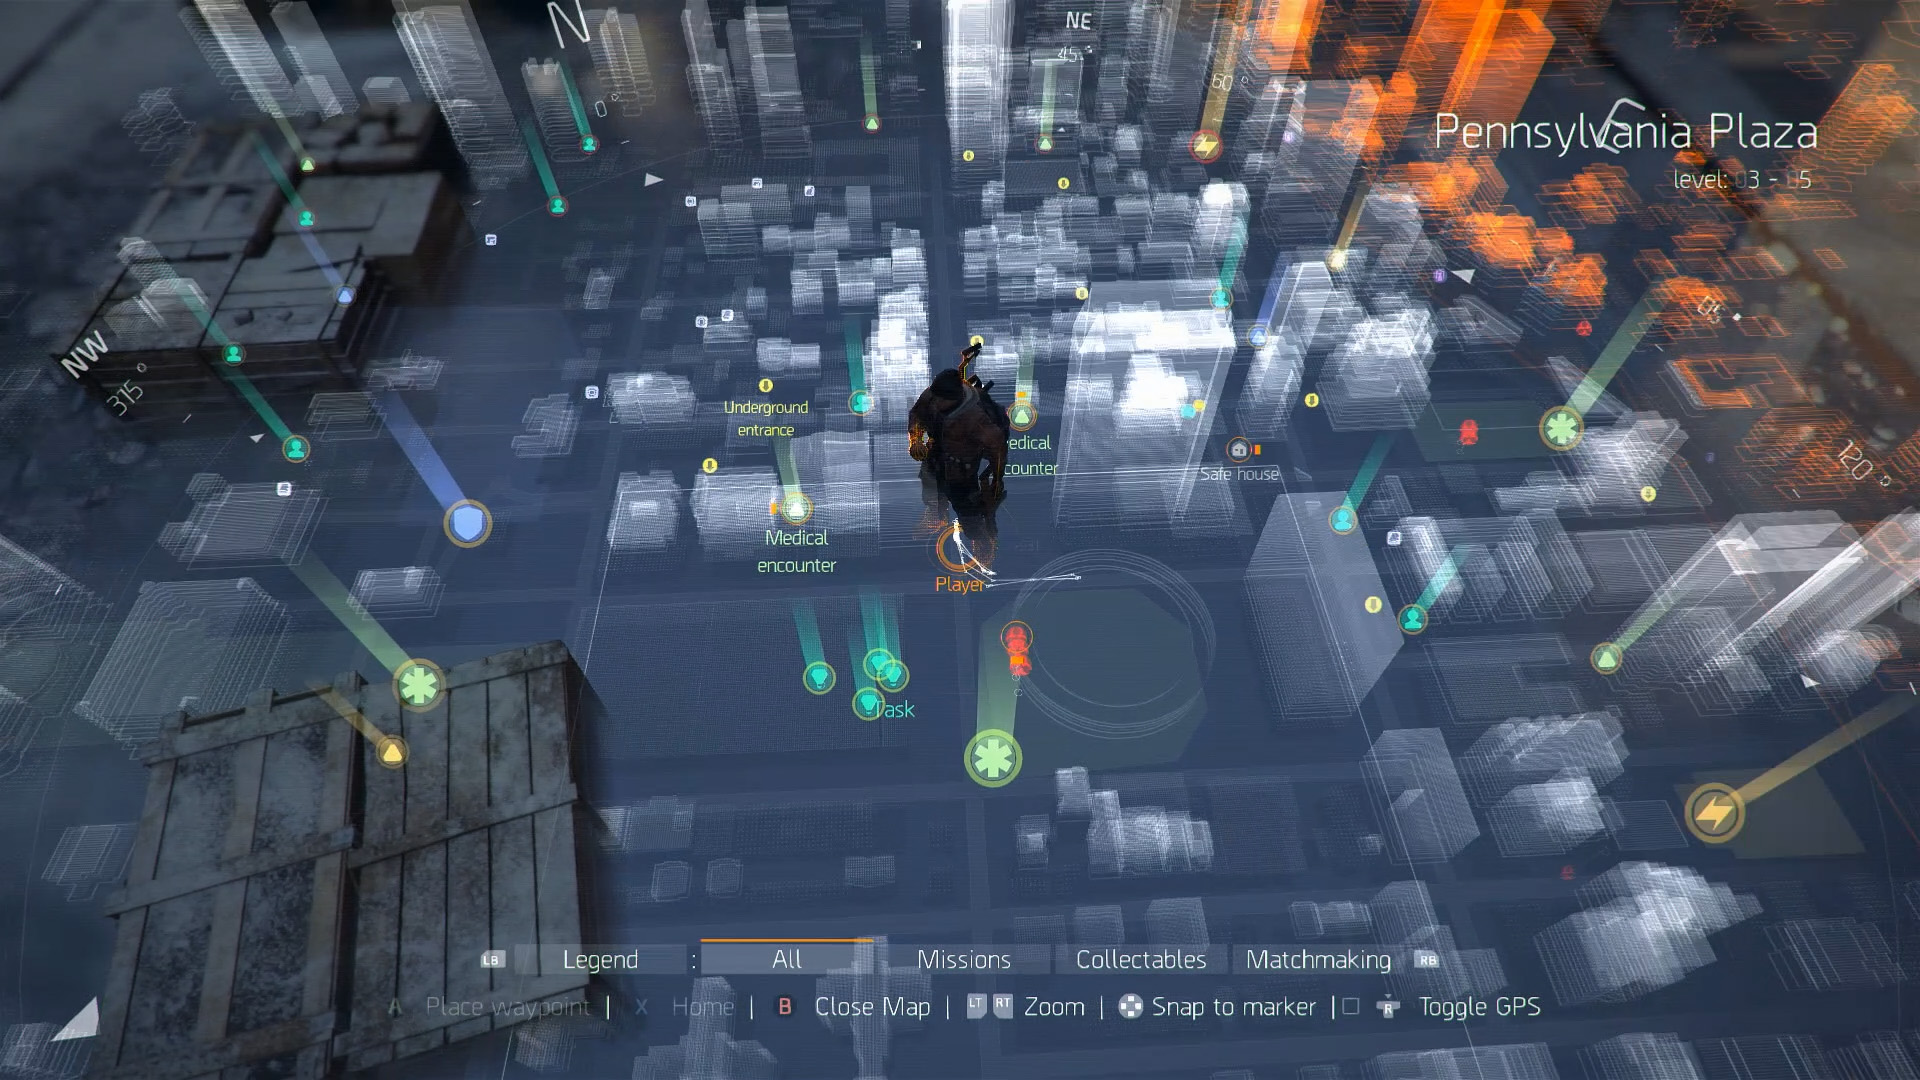
\includegraphics[width=0.95\textwidth]{figures/the_division_megamap.jpg}
	\caption{Die \enquote{Megamap} aus \emph{\glsentrylong{TCTD}}. Symbole zeigen Missionsziele, Gegenstände und wichtige Orte im Spiel. \quelle{\cite{MYDIVISION.NET2014}}}
	\label{fig:megamap}
\end{figure}
Eine Karte der Umgebung wird mit relevanten Spielobjekten und Ortsnamen \emph{im Spiel} als \gls{AR}-Interface um den Charakter herum angezeigt.
Die Karte erlaubt dem Spieler unter anderem, Wegpunkte festzulegen (Navigation), interessante Punkte in der Umgebung anzuzeigen und zu filtern (Exploration) sowie die Ansicht durch Verschieben und Zoomen der Karte anzupassen.

% Aufgabenstellung
Da nicht unmittelbar klar ist, ob sich das Konzept der Megamap in die reale Welt übertragbar ist, ergibt sich die zentrale Fragestellung dieser Arbeit:
\begin{quote}
\itshape
Ist eine \gls{AR}-Megamap geeignet, um Nutzer bei der Exploration von \emph{realen} Umgebungen zu unterstützen?
\end{quote}
Um diese Frage zu beantworten wird in dieser Masterarbeit die Entwicklung einer prototypischen Kartenanwendung mit einem \gls{HMD} als Zielplattform beschrieben.
Die Karte soll dem Nutzer (wie in \gls{TCTD}) eine virtuelle 3D-Karte anzeigen.
Sie soll dabei in die tatsächliche Umgebung des Nutzers eingebettet werden, sodass dieser sich darin umherbewegen kann.
Über eine Gestensteuerung soll der Nutzer mit der Karte interagieren und Explorationsanfragen stellen können.
Schließlich soll die Effektivität des Prototypen in Bezug auf die zuvor genannte Fragestellung durch eine Evaluation bestätigt werden.

\section{Struktur der Arbeit}
\label{sec:struktur}
% TODO Struktur der Arbeit beschreiben (am Ende).
{\itshape In diesem Abschnitt wird später die komplette Struktur der Arbeit beschrieben (ca. 1--2 Sätze pro Kapitel.) \dots}

%
\cleardoublepage